\documentclass[11pt]{article}
\usepackage[margin=1in]{geometry}
\usepackage[T1]{fontenc}
\usepackage{lmodern}
\input{ot1lmr.fd}
\DeclareFontShape{T1}{lmr}{m}{n}{<-> ec-lmr10}{}
\DeclareFontShape{T1}{lmr}{m}{it}{<-> ec-lmri10}{}
\DeclareFontShape{OT1}{lmr}{m}{n}{<-> rm-lmr10}{}
\input{omllmm.fd}
\DeclareFontShape{OML}{lmm}{m}{it}{<-8.5> lmmi8 <8.5-> lmmi10}{}
\input{omslmsy.fd}
\DeclareFontShape{OMS}{lmsy}{m}{n}{<-8.5> lmsy8 <8.5-> lmsy10}{}
\usepackage{amsmath,amssymb,booktabs,graphicx,microtype}
\usepackage[hidelinks]{hyperref}
\urlstyle{same}
\setlength{\emergencystretch}{2em}
\clubpenalty=10000\widowpenalty=10000
\title{Shaping Gap Benchmark VI:\\A Second Compatible Neural Acquisition\\Through Program-Contract Interfaces}
\author{Nathaniel Oh \and Paul Attie}
\date{November 13, 2026}
\begin{document}
\maketitle
\begin{abstract}
Can an already improved component runtime acquire another neural improvement while keeping its previous programs and processing quality usable? We extend an accepted frozen-component runtime with bounded native-port recruitment and one shared canonical observation interface. A screening study over six inherited contexts scales candidate inventories from 64 to 512 while retaining at most four recruited ports; the largest guided pool yields fresh terminal gains in four contexts, but the prespecified already-improved chain stalls. Its candidate quality gains frequently fail preservation. A prospective follow-up acquires shared interfaces against the retained programs' source contracts and jointly selects an execution/interface pair. On two untouched terminal streams, the selected pair improves nonlinear temporal quality by 33.24\% and 49.60\% relative to the already improved reference, retaining all six protected program instances. Feature-interface control gains are 20.52\% and 27.61\%; interface-only control retains baseline. The successful construction adds one original pretrained component and keeps a 600-value shared affine map. One additional acquisition is confirmed; the stronger two-additional-acquisition criterion is not met. A separate chronological appliance-energy transfer test yields 0.56\% lower one-hour RMSE, a 2.22\% ten-minute regression and a stronger classical reference. All controls, failed attempts, source-label access and lifecycle costs are recorded. The result establishes a second finite compatible acquisition and a measurable route from component recruitment to application-specific development.
\end{abstract}

\section{From one accepted improvement to another}
Checkpoint V supplied an experience-selected component runtime that executes original pretrained neural fragments without invoking the source transformer graph~\cite{sg5}. Its accepted 0.6B-derived context 151003 improved a finite numerical temporal-processing score on fresh streams while retaining its eligible old programs. This checkpoint starts from that exact accepted state. The question is whether another neural construction can improve it while keeping the first improvement and its programs usable.

We study a coupled object: the acquired execution change and the acquired shared observation interface. Improving the native state evolution can also change the observations expected by earlier programs. A feature-alignment map and a program-contract map express different acquisition objectives for the same interface. Old readout arrays remain fixed in both cases.

The contribution is a second compatible acquisition over frozen native components, with recruitment work, a fixed active-port cap, a fixed-size shared map, prospective fresh testing and an application transfer check. It builds on the acquired execution/interface pair of Checkpoint IV~\cite{sg4} and the component execution of Checkpoint V. The three studies are kept distinct: P64 diagnoses recruitment and preservation; P65 tests contract-directed interface acquisition on new streams; P66 tests application transfer without adapting the retained controllers.

\begin{figure}[ht]\centering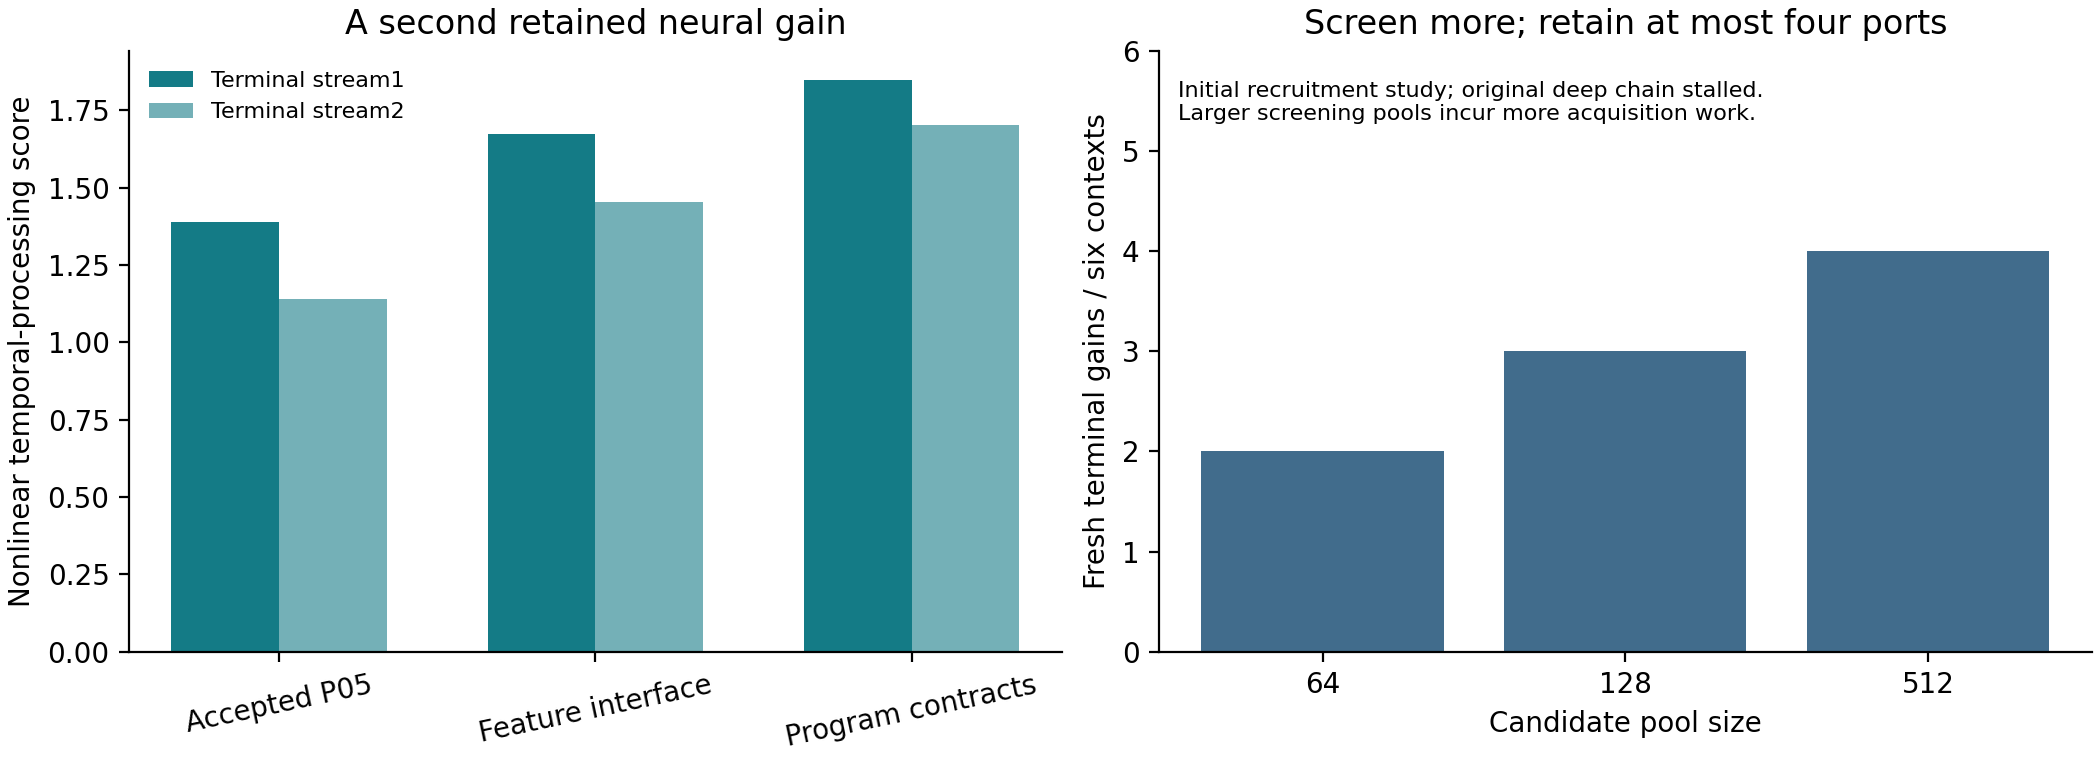
\includegraphics[width=\linewidth]{checkpoint-overview.png}
\caption{Left: terminal quality from the already accepted Checkpoint V runtime and two acquired successors. Right: P64 screening at increasing pool sizes; all six contexts and baseline fallbacks are included. Larger pools incur additional acquisition work.}\label{fig:overview}
\end{figure}

\section{Bounded recruitment over fixed pretrained components}
\subsection{Inherited runtime and native ports}
The inherited runtime retains 24 sampled SwiGLU fragments per context, two stages of response-guided execution, an eight-dimensional recurrent state and 24 observations. Pretrained gate/up/down/normalization arrays, input coordinates, component-response interfaces and original return matrices are unchanged. The source transformer graph, attention and token-generation path are absent. Numerical materialization and full-coordinate fidelity are documented in Checkpoint V.

For each of the six inherited model/context cells, we extract 512 additional physical units from the same pinned source checkpoints, excluding the initial 24. The two models are Qwen3-0.6B and Qwen3-1.7B. Source units are sampled without task outcomes. Pool extraction uses guarded original primitives, records complete preparation time and peak RSS, and preserves original parameter digests. The immutable pool is an external substrate archive, distinct from retained controller state.

For a port $i$, let $a_i(s)$ be its original SwiGLU amplitude on the inherited affine input driven by the eight-state vector and scalar stimulus. A native response contrast is
\begin{equation}
 r_i(s)=a_i(s)-a_i(0)-D a_i(0)s.
\end{equation}
It removes the measured anchor constant and first-order part. The native down column, projected through the accepted return, supplies an eight-state write direction $b_i$. With recruited edges $E$, state execution becomes
\begin{equation}
 z_{t+1}=C_1\bigl(F([z_t;0.2u_t])-F(0)\bigr)
       +\sum_{i\in G_t(E)}\alpha_i b_i r_i([z_t;0.2u_t]).
\end{equation}
The first term is the accepted component runtime, not a transformer invocation. At most four recruited ports are retained; at most two execute per step. Source-calibrated signed fractions $\{-5\%,-2\%,+2\%,+5\%\}$ define supplied proposal strengths. Native rows stay fixed; edge identity, coefficient and observation interface are acquired.

\subsection{Local interfaces and streamed screening}
Candidate pools are read in 16-row chunks. Guided screening uses the current unmet-target residual propagated through frozen readout state sensitivities. A candidate scores by normalized alignment of its contrast response with that local loss direction. This is an immediate sensitivity heuristic, not a full recurrent adjoint. Random recruitment samples two candidate identities without screening the whole pool; resident-only screening uses the original 24 fragments. Their different query costs are charged.

Only the two shortlisted ports acquire local quadratic response interfaces, from 64 native value/partial observations in nine input coordinates. Interface cost therefore depends on shortlisted ports and the fixed local coordinate dimension, rather than a dense polynomial over the whole inventory. Their predicted contrast magnitudes rank the retained ports when more than two are present. The successful P65 runtime retains one extra port, so competition between multiple recruited ports and eviction are not exercised by that success.

The four-slot cap includes a supplied replacement rule: if full, propose replacing the source-smallest-RMS edge and evaluate the resulting obligations. No claim of indefinitely growing capability follows from that finite cap. Program-library storage, acquisition workspace and whole-process memory are separately measured.

\section{Preservation in a common observation space}
All programs consume a canonical space corresponding to the accepted Checkpoint V observations. A child-to-parent raw affine interface composes with the parent's interface:
\begin{equation}
 A_{c\to0}=A_{c\to p}A_{p\to0},\qquad
 b_{c\to0}=b_{c\to p}A_{p\to0}+b_{p\to0}.
\end{equation}
The shared deployed map contains $24\times24+24=600$ numerical values regardless of cycle count. The initial legacy adapter connects canonical observations to the preceding programs' original coordinates. Program coefficients are not rewritten or refitted. Newly acquired assessment programs are separately retained and charged; this does not bound an unlimited archive of programs.

Preservation has two obligations. Every fixed eligible program must retain $R^2\geq0.5$. In addition, each retained library's nonlinear processing quality must stay within 1\% of its paired parent reference. The original accepted library is also checked against a fixed Checkpoint V reference, preventing gradual loss through a moving reference alone. These are finite empirical contracts on declared input streams.

The temporal assay has 143 normalized Legendre-product functions through degree four, including 109 multi-lag nonlinear targets~\cite{dambre}. Quality $Q$ sums positive held-out $R^2$ over those 109. New assessment heads fit the same source examples on baseline and candidate. Thus an execution gain is measured against an equal-source-refitted baseline, while older frozen programs independently measure retained access.

Each round uses source experience, two feedback streams and then two untouched validation streams. Feedback selects a pair; its programs, map and controller are locked before validation. A fresh pass commits that state for the next round. A fresh failure rolls back, preserving the failed result and its costs. Prior round outcomes become explicit experience for later rounds. After the final round, controller states and equally exposed terminal heads are sealed before two new 2,048-step terminal streams.

\section{P64: recruitment scales, the improved chain stalls}
P64 compares guided pools of 64, 128 and 512, random selection from 128, and resident-only selection. All six contexts execute one round per arm. The already improved 0.6B context 151003 executes five rounds per arm, prespecified from its published earlier result. There are 50 round cells in total.

\begin{table}[ht]\centering\small\begin{tabular}{lrrrr}
\toprule
Arm & Terminal gains & $\Delta Q_1$ & $\Delta Q_2$ & Port queries \\
\midrule
guided-64 & 2/6 & +0.12817 & +0.12212 & 1,164,712 \\
guided-128 & 3/6 & +0.31781 & +0.31108 & 1,833,768 \\
guided-512 & 4/6 & +0.43056 & +0.42208 & 5,782,824 \\
random-128 & 3/6 & +0.36832 & +0.39749 & 542,268 \\
resident & 3/6 & +0.32919 & +0.34294 & 767,768 \\
\bottomrule
\end{tabular}

\caption{P64 terminal results across six contexts. Work counts include screening and recruited-port queries; the base component runtime is counted separately. No arm adds a retained gain on the prespecified already-improved deep chain.}\label{tab:recruitment}
\end{table}

The 512-pool arm yields terminal gains in four of six contexts, versus three for 128 and two for 64. Random and resident controls each have three. More screening produces more opportunities in this finite cohort, with greater discovery work; this is not uniform economical superiority over the cheaper controls.

The already improved chain has no accepted additional gain in any arm. Of its 200 development candidates, 112 improve own processing quality in both blocks and 110 of those preserve the fixed reliable program IDs, but only nine preserve the stronger prior-quality contract. Across the complete study, 288/400 improve quality in both feedback blocks; 66 of those meet prior-quality preservation. Source opportunities and fresh retained acquisitions are reported separately.

This result motivates the next intervention at compatibility acquisition. P65 retains the preservation tests and tests an interface that is acquired against what the old programs must compute. P64 outcomes remain development evidence for that decision, not P65 validation.

\section{P65: acquire the interface against program contracts}
\subsection{One shared program-directed map}
Feature transport fits paired neural coordinates with a ridge identity prior. The new alternative fits a shared map using source input-history targets evaluated through the unchanged old programs. This explicitly adds functional target labels to interface acquisition; it is not the label-free transport of earlier checkpoints. These targets are computed from numerical input history, rather than supplied English descriptions or a hosted teacher.

Let $X$ contain standardized child features plus a constant column, $P$ be the shared affine coefficients in standardized canonical coordinates, and $Z$ be the paired parent canonical features. For retained program library $\ell$, let $W_\ell$ and $c_\ell$ express its unchanged outputs from standardized canonical coordinates. We minimize
\begin{equation}
 \omega\|XP-Z\|_F^2+
 \sum_\ell\|(XPW_\ell+c_\ell-Y)D_\ell\|_F^2+
 \lambda\|P-P_0\|_F^2.
\end{equation}
$D_\ell$ scales target variances and gives fixed eligible programs fourfold squared-loss weight. The normal equation has the form
\begin{equation}
 (X^\top X)PM+\lambda P=R.
\end{equation}
An eigendecomposition of the 24-dimensional output weight $M$ reduces this to small ridge solves. We supply feature weights $\{0.01,0.1,1\}$ and ridge fractions $\{0.001,0.01\}$. Feedback jointly selects among the execution/interface pairs. The construction uses established weighted regression; the empirical question is whether the acquired pair enables a retained second gain.

\subsection{Controls and information boundaries}
The feature arm retains the original paired-feature interface. The contract arm offers that map and six program-directed alternatives per physical construction. The interface-only arm offers the same program-directed alternatives while leaving neural execution unchanged. Identical physical constructions share their exact native trajectories within an arm; alternative map fitting and program execution are charged, with no extra native queries invented for those views.

All three arms execute five rounds on the prespecified already improved context. Source, feedback, fresh and terminal seeds are new relative to P64. Every old program, quality floor, slot cap and rollback rule remains unchanged. New assessment heads have matched source exposure. The selected source map is fixed before fresh outcomes, and all terminal controllers are fixed before final terminal inputs.

\subsection{A second neural gain survives terminal reuse}
Both the feature and contract arms accept one neural recruitment in round three; their other four rounds retain baseline or roll back. Both recruit pool port 38. The feature arm selects a $+2\%$ connection; the joint contract arm selects $+5\%$ with an acquired program-directed interface. The interface-only arm accepts no change.

\begin{table}[ht]\centering\small\begin{tabular}{lrrrr}
\toprule
Runtime & $Q_1$ & $Q_2$ & Relative gains & Old \\
\midrule
Accepted Checkpoint V & 1.38792 & 1.13904 & -- & 4/4 \\
feature & 1.67273 & 1.45352 & 20.52\% / 27.61\% & 6/6 \\
contract & 1.84921 & 1.70404 & 33.24\% / 49.60\% & 6/6 \\
interface only & 1.38792 & 1.13904 & 0.00\% / 0.00\% & 4/4 \\
\bottomrule
\end{tabular}

\caption{P65 common terminal streams. The reference is the already improved Checkpoint V runtime, evaluated on these same inputs. Six protected program instances belong to three frozen libraries, not six distinct target functions.}\label{tab:second}
\end{table}

The contract pair changes terminal quality from $(1.38792,1.13904)$ to $(1.84921,1.70404)$: gains of 33.24\% and 49.60\%, retaining all six protected program instances and the aggregate quality obligations. The feature-interface control reaches $(1.67273,1.45352)$, gains of 20.52\% and 27.61\%, also retaining all six instances. The reference is a small finite processing score; these percentages are not general language-model accuracy improvements.

Within the contract arm, the identical $+5\%$ physical connection is also evaluated with the feature interface. Its fresh own-quality scores are $(1.53506,1.75407)$, versus $(1.78247,2.07779)$ through the program-directed map. The corresponding frozen legacy-library qualities change from $(0.91165,0.85676)$ to $(0.93939,0.89108)$; the selected pair meets the preserved obligations. These are paired outcomes for the same physical construction, rather than an attribution based only on different selected doses.

The successful controller retains one extra native port, a fixed 600-value map and 1,102,272 bytes of conservatively counted runtime/program arrays under the supplied 8 MiB payload cap. Whole-process peak RSS is larger and reported separately. P63 supplies the first accepted improvement and P65 the second; within P65 only one additional neural acquisition is accepted. The stronger criterion of two additional acquisitions is not met, and active-slot eviction is not exercised.

\section{P66: chronological energy-forecast transfer}
The application study freezes all controllers and fits new forecast readouts on the public UCI Appliances Energy Prediction series~\cite{uci}. The series has 19,735 ten-minute measurements. We use prior/current appliance consumption only, with a training-only log transform and scaling. The first 60\% trains the readouts, the next 20\% is validation without tuning, and the final 20\% is untouched testing. Forecast targets never cross partition boundaries; recurrent state carries forward causally.

The contract controller is designated prospectively, not selected using application performance. Controls include the feature and interface-only successors, the earlier component baseline, the accepted Checkpoint V runtime, 64-lag ridge autoregression, persistence and a daily seasonal reference. The new readouts and classical fitted baseline receive the same forecast target examples. No neural execution or pretrained parameter is adapted on the application data.

\begin{figure}[ht]\centering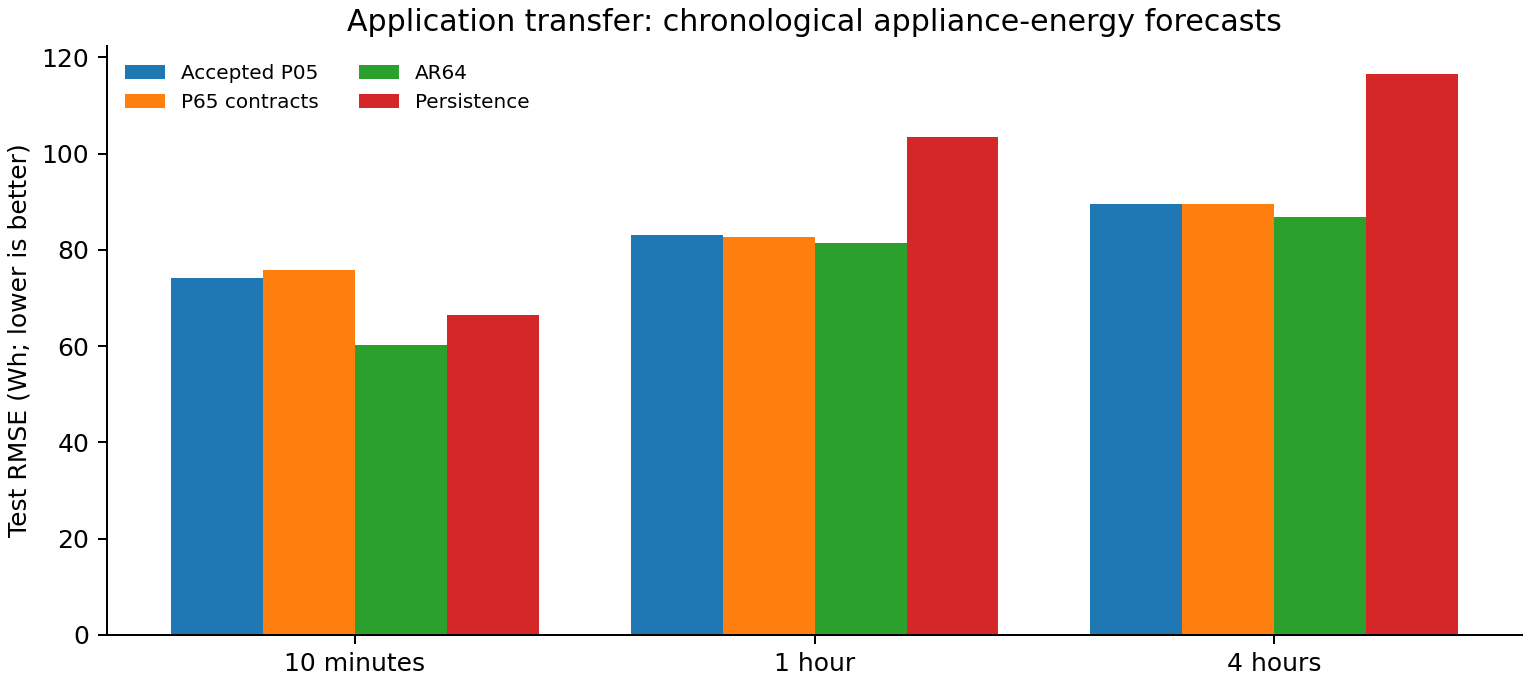
\includegraphics[width=.97\linewidth]{application-results.png}
\caption{Application test RMSE. The retained numerical construction gives a small one-hour improvement; short-horizon regression and the stronger AR64 reference remain visible.}\label{fig:application}
\end{figure}

\begin{table}[ht]\centering\small\begin{tabular}{lrrr}
\toprule
Forecaster & 10 minutes & 1 hour & 4 hours \\
\midrule
Before first gain & 71.3236 & 83.2283 & 89.6541 \\
Accepted Checkpoint V & 74.2173 & 83.1373 & 89.5248 \\
P65 feature interface & 73.5964 & 83.0632 & 89.6307 \\
P65 program contracts & 75.8649 & 82.6682 & 89.5168 \\
P65 interface only & 74.2173 & 83.1373 & 89.5248 \\
AR64 & 60.1605 & 81.4353 & 86.8620 \\
Persistence & 66.4713 & 103.4557 & 116.6360 \\
Daily seasonal & 110.2941 & 109.7830 & 109.0170 \\
\bottomrule
\end{tabular}

\caption{Chronological test RMSE in Wh, lower is better. Full MAE, validation metrics, per-example predictions and paired resampling results are released.}\label{tab:application}
\end{table}

One-hour RMSE changes from 83.1373 to 82.6682 Wh, a 0.564\% reduction. The prespecified paired daily-block bootstrap interval for relative improvement is $[0.101\%,1.175\%]$. Ten-minute RMSE increases 2.220\%, and four-hour improvement is approximately 0.009\%. AR64 is stronger at all three horizons. The primary requirement of at least 1\% one-hour improvement with no more than 1\% regression elsewhere is not met.

This distinguishes transferable representation change from demonstrated operational advantage. The next application acquisition can use forecast requirements directly and protect the short-horizon consumer while pursuing a longer-horizon gain. The present study supplies the actual error scales, competitive reference and regression obligation for that work, without claiming measured commercial savings.

\section{Lifecycle accounting and independent checks}
P64 takes 175.41 seconds in the recorded CPU environment, with peak RSS 88.92 MiB. P65 takes 48.79 seconds, with peak RSS 150.73 MiB. P66 takes 5.27 seconds, with peak RSS 159.45 MiB. These are complete numerical-study measurements, not per-request production latencies. P64's maximum measured screening workspace is 660,864 bytes. Whole-process memory, retained payload and original-checkpoint preparation are different quantities.

Recruitment-pool preparation takes 6.38 seconds with peak process RSS 1.47 GiB; 3,072 additional ports are extracted across the two model sizes and three contexts. Native preparation, source profiles, screening, unused candidate pairs, interface fitting, failed selections, rollbacks, program libraries and terminal tests are charged. Inherited Checkpoint V and earlier development are carried as historical work; pretraining is inherited and unmeasured, rather than free. Electrical energy is not measured.

The original P64 engineering launch stops before feedback because exact equality was requested between the parent executed alone and in a batch. The maximum feature discrepancy is $4.24\times10^{-16}$ and states are identical. The recorded retry uses the inherited native numerical tolerance, preserves the failure and changes no scientific criterion. The complete initial failed-process duration was not captured. P65 progress metadata retains an inherited expected-context count of 18; the protocol and completed summary correctly specify three contexts/arms. This display-count defect changes no outcome or stopping condition.

Independent replay checks 6,540 P64 score vectors and 650 seals, then 5,572 P65 vectors and 459 seals; maximum score discrepancies are below $1.56\times10^{-15}$. It independently refits source heads, reconstructs every feedback choice, fresh acceptance, rollback and terminal gain. A separate forward-loss stationarity check verifies all 300 acquired program-contract maps with maximum relative residual $5.91\times10^{-13}$. Direct original-width component arithmetic checks 8,320 source responses from 130 local interfaces, with maximum relative value/partial errors $1.22\times10^{-13}$ and $6.12\times10^{-15}$. Application replay reproduces every prediction and all 48 metric rows exactly and verifies training-only preprocessing and sealed readouts.

\section{Building blocks and the research direction}
Temporal processing measurements~\cite{dambre}, frozen pretrained reuse~\cite{lu} and trainable stitching~\cite{stitch} provide foundations. Recent work also adapts frozen-model execution topology~\cite{selfmorph} and connects whole frozen models through learned latent projections~\cite{deadweights}. Our measured contribution is a second native-component acquisition with jointly acquired program compatibility, bounded recruitment, independent fresh terminal validation and a prospective application boundary.

A useful next acquisition must repay screening, preserve what earlier programs compute and increase task-relevant processing. The current result supplies a two-improvement chain and identifies where the next obligations lie: repeated successful acquisitions beyond this second gain, reliable replacement within a full active bank, and application-directed contracts that produce competitive error and lifecycle economics. The public artifact retains the successful and unsuccessful legs of that progression.

\appendix
\section{Declared scope and reproduction}
P64 contains 30 first-round model/context/arm cells plus 20 deep continuation rounds; P65 contains three five-round arms. All repeated observations share the declared source models and input families. A deep chain selected from a published prior success supports a scoped continuation result, not an independent population estimate.

The companion includes source, protocols, complete candidate outcomes, all programs/maps, frozen parameter provenance, acquisition work, failed criteria and replay. CPU execution uses the compiled parameter-backed components; original checkpoints are needed only for re-extraction. Public code supplies cached replay and a fresh acquisition workspace. Original papers and data remain at their previous checkpoint paths. The source-model revisions and model terms are inherited from Checkpoint V. The UCI series is redistributed with its CC BY 4.0 attribution. No arXiv identifier is assigned.

\begin{thebibliography}{9}\footnotesize\setlength{\itemsep}{0pt}\raggedright
\bibitem{sg4} N. Oh and P. Attie. Shaping Gap Benchmark IV: Experience-Acquired Execution and Compatibility Reuse. Repository paper, 2026. \url{https://github.com/calysteon/shaping-gap-benchmark/tree/main/checkpoints/04-experience-acquired-reuse}.
\bibitem{sg5} N. Oh and P. Attie. Shaping Gap Benchmark V: Learned Component Execution Beyond the Transformer Graph. Repository paper, 2026. \url{https://github.com/calysteon/shaping-gap-benchmark/tree/main/checkpoints/05-component-learning-cycle}.
\bibitem{dambre} J. Dambre, D. Verstraeten, B. Schrauwen and S. Massar. Information Processing Capacity of Dynamical Systems. \emph{Scientific Reports} 2, 514, 2012. \url{https://doi.org/10.1038/srep00514}.
\bibitem{uci} L. Candanedo. Appliances Energy Prediction. UCI Machine Learning Repository, 2017. \url{https://doi.org/10.24432/C5VC8G}. CC BY 4.0.
\bibitem{lu} K. Lu, A. Grover, P. Abbeel and I. Mordatch. Pretrained Transformers as Universal Computation Engines. 2021. \url{https://arxiv.org/abs/2103.05247}.
\bibitem{stitch} Y. Bansal, P. Nakkiran and B. Barak. Revisiting Model Stitching to Compare Neural Representations. \emph{NeurIPS}, 2021. \url{https://arxiv.org/abs/2106.07682}.
\bibitem{selfmorph} J. Wu, Y. Guo and S.-T. Xia. Compute Has Shape: Self-Morphing the Internal Computation of Frozen LLMs. 2026. \url{https://arxiv.org/abs/2610.38382}.
\bibitem{deadweights} M. Armstrong, N. Ayoobi and A. Mukherjee. Dead Weights, Live Signals: Feedforward Graphs of Frozen Language Models. 2026. \url{https://arxiv.org/abs/2604.08335}.
\end{thebibliography}
\end{document}
